% Load preamble
\documentclass[../main.tex]{subfiles}

\begin{document}
	
\subsection{Úvodný príklad}
Uvažujme nelineárny systém, opísaný stavovými rovnicami \ref{eqn:Rovnica1}, ktorého bloková schéma je zobrazená na obrázku \ref{fig:BlokovaSchemaPr1}. 

\begin{equation}
	\begin{aligned}
	\dot{x_1} &= x_1^2 + x_2 - x_1 \\
	\dot{x_2} &= u - x_1 - x_2 \\
	\end{aligned}
	\label{eqn:Rovnica1}
\end{equation}



Na riadenie nelineárneho systému (rovnica \ref{eqn:Rovnica1}), použijeme metódu vstupno-stavovej spätnoväzobnej linearizácie (obrázok \ref{fig:MetodaVS}), tak aby sme dosiahli požadovanú hodnotu $r$.
\begin{figure}[H]
	\begin{center}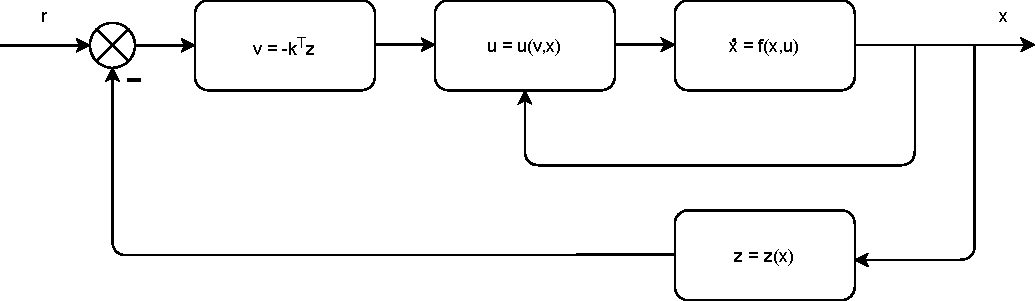
\includegraphics[scale=0.8]{MVSlin.pdf}\end{center}
	\caption{Metóda vstupno-stavovej spätnoväzobnej linearizácie}
	\label{fig:MetodaVS}
\end{figure}

Postup pri metóde vstupno-stavovej spätnoväzobnej linearizácie je nasledovný.

\subsubsection{Prvý krok - určenie transformačných vzťahov}
Najskôr si určíme transformačné vzťahy, tzn. určíme vektor $r$.
\begin{equation}
	\begin{aligned}
        z_1 &= x_1 \\
		z_2 &= x_1^2 + x_2 \\
	\end{aligned}
	\label{eqn:TransformacneVztahy}
\end{equation}

\subsubsection{Druhý krok - transformácia systému}
Následne transformujeme zadaný nelineárný systém (rovnica \ref{eqn:Rovnica1}), pomocou nájdených transformačných vzťahov (rovnica \ref{eqn:TransformacneVztahy}).
\begin{equation}
	\begin{aligned}
	\dot{z_1} &= \dot{x_1} = z_2 - z_1 \\
	\dot{z_2} &= 2x_1\dot{x_1} + \dot{x_2} \\
	          & = 2x_1(x_1^2 + x_2 - x_1) + u - x_1 - x_2 \\
	          & = 2z_1(z_2 - z_1) + u - z_1 - z_2 + z_1^2\\
	          & = u - z_1^2 + 2z_1z_2 - z_1 - z_2 \\
	\end{aligned}
	\label{eqn:TransformovanySystem}
\end{equation}
Aby sme dosiahli lineárny transformovaný systém, zavedieme novú premennú $v$.
\begin{equation}
	\begin{split}
	 v = u - z_1^2 + 2z_1z_2 - z_1 - z_2 \\
	\end{split}
	\label{eqn:SubsV}
\end{equation}
Z transformovanej sústavy získame vzťah pre nelineárne riadenie, akčný zásah $u$.
\begin{equation}
	\begin{gathered}
		u = v + z_1^2 - 2z_1z_2 + z_1 + z_2\\
	\end{gathered}
	\label{eqn:Noveu}
\end{equation}
Zavedením novej premennej sme získali nový transformovaný lineárny systém.
\begin{equation}
	\begin{aligned}
	\dot{z_1}  &= z_2 - z_1 \\
	 \dot{z_2} &= v \\
	\end{aligned}
	\label{eqn:TransformovanySystem}
\end{equation}

\subsubsection{Tretí krok - návrh lineárneho stavového regulátora}
Po získaní lineárneho systému môžeme zaviesť lineárny stavový regulátor (rovnica \ref{eqn:LinReg}).
\begin{equation}
	\begin{split}
		v = k_1z_1 + k_2z_2 \\
	\end{split}
	\label{eqn:LinReg}
\end{equation}
Lineárny systém s regulátorom bude vyzerať nasledovne: rovnica \ref{eqn:TransformovanySystemSRegulatorom}. 
\begin{equation}
	\begin{aligned}
	\dot{z_1}  & = z_2 - z_1 \\
	 \dot{z_2} & = k_1z_1 + k_2z_2 \\
	\end{aligned}
	\label{eqn:TransformovanySystemSRegulatorom}
\end{equation}
Na vypočítanie parametrov regulátora a nastavenie dynamiky systému potrebujeme odvodiť charakteristickú rovnicu systému.
Na získanie charakteristickej rovnice potrebujeme získať maticu $A$.
\begin{equation}
\begin{aligned} 
 A  & = \begin{bmatrix} \frac{\partial \dot{z_1}}{\partial z_1}& \frac{\partial \dot{z_1}}{\partial z_2}\\ \frac{\partial \dot{z_2}}{\partial z_1}&\frac{\partial \dot{z_2}}{\partial z_2} \end{bmatrix}_{|_{z_1 = z_2 = 0}} \\
 & = \begin{bmatrix} -1 & 1\\ k_1 & k_2 \end{bmatrix} \
 \end{aligned}
 \label{eqn:A}
\end{equation}
Charakteristickú rovnicu získame z rovnice \ref{eqn:CHR}.
\begin{equation}
\begin{aligned} 
 |\lambda I - A| & = 0\\
|\lambda I - A| & = \begin{bmatrix} \lambda +1 & -1\\ -k_1 & \lambda -k_2 \end{bmatrix} \\
|\lambda I - A| & = (\lambda + 1)(\lambda - k_2) - k_1\\
\lambda^2 - \lambda(k_2+1) - k_1 &= 0\\ 
\end{aligned}
\label{eqn:CHR}
\end{equation}

Vieme, že korene charakteristickej rovnice musia ležať v zápornej polrovine. Preto si zvolíme korene $\lambda_1 = -1$,$\lambda_2 = -2$, pomocou ktorých získame parametre $k_1,k_2$ (rovnica \ref{eqn:Korene}).
\begin{equation}
\begin{aligned} 
\lambda^2 - \lambda(k_2+1) - k_1 & = (\lambda + 1)(\lambda + 2)\\ 
\lambda^2 - \lambda(k_2+1) - k_1 & = \lambda^2 + 3\lambda + 2\\ 
k_1 &= -2\\
k_2 &= -4\\
\end{aligned}
\label{eqn:Korene}
\end{equation}

\subsubsection{Overenie výsledkov}
Výsledky overíme simulačne pomocou schémy na obrázku \ref{fig:PrikladsRiadenim}.
\newpage
\begin{figure}[H]
	\begin{center}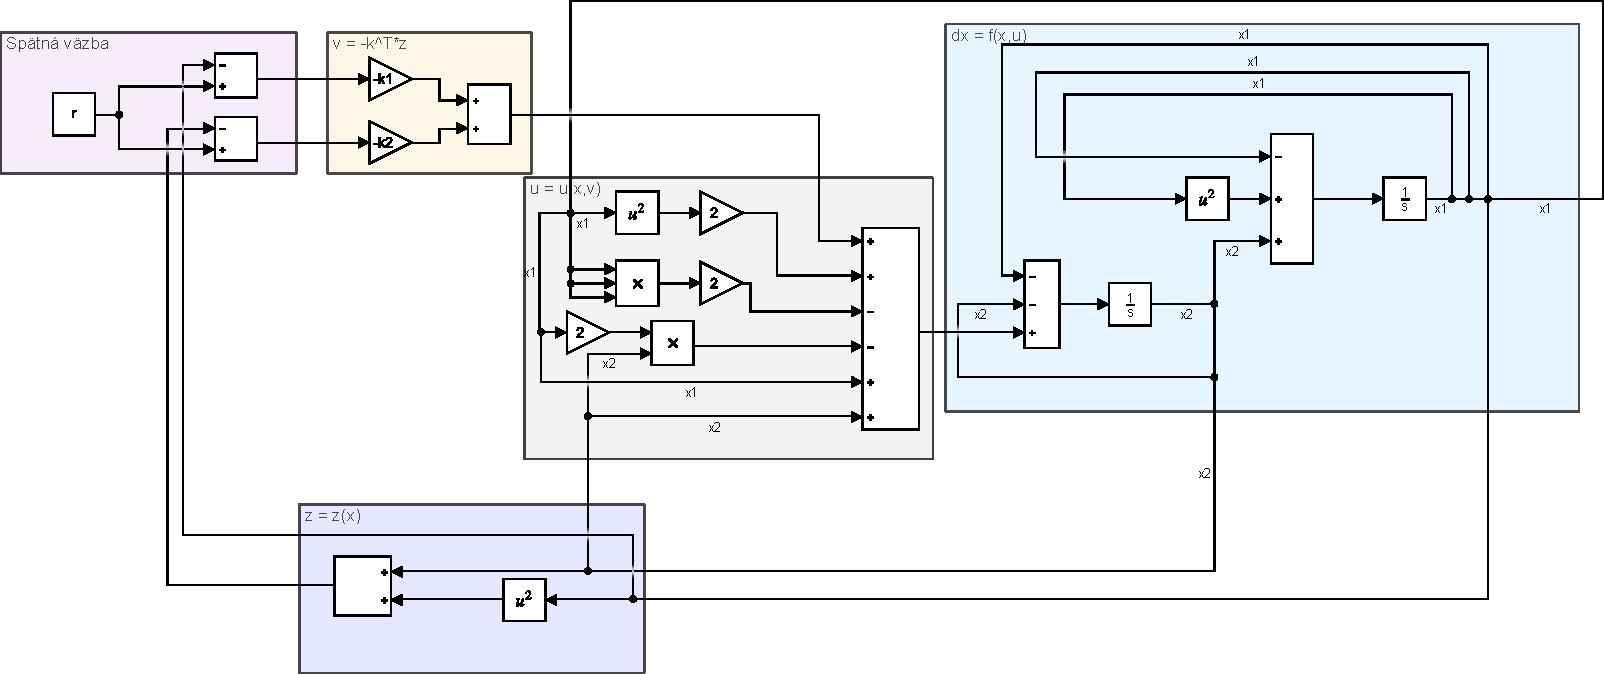
\includegraphics[scale=0.8,angle=90]{Rovnica1MVS.pdf}\end{center}
	\caption{Bloková schéma systému s nelineárnym riadením}
	\label{fig:PrikladsRiadenim}
\end{figure}

Z výsledkov simulácie, ktoré sú zobrazené na obrázkoch \ref{fig:Vysledok1}, \ref{fig:Vysledok2}, môžeme vidieť, že s pomocou navrhnutého riadenia pre nelineárny systém sme dokázali dosiahnuť požadovanú hodnotu $r$.
\begin{figure}[!htb]
   \begin{minipage}{0.46\textwidth}
     \centering
     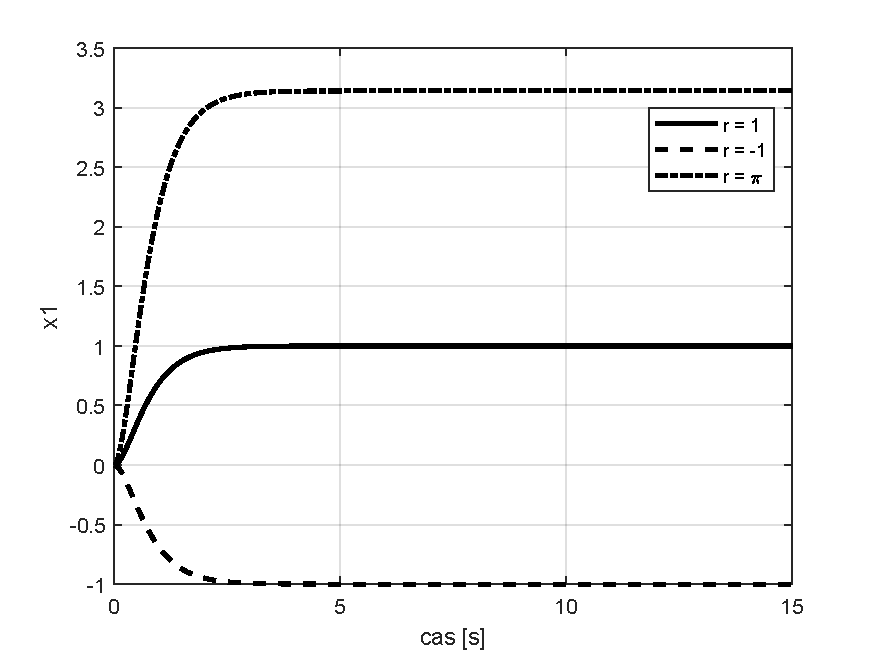
\includegraphics[width=1\linewidth]{x.pdf}
     \caption{Priebeh stavovej premennej $x_1$ s nelineárnym riadením}
	\label{fig:Vysledok1}
   \end{minipage}\hfill
   \begin{minipage}{0.46\textwidth}
     \centering
     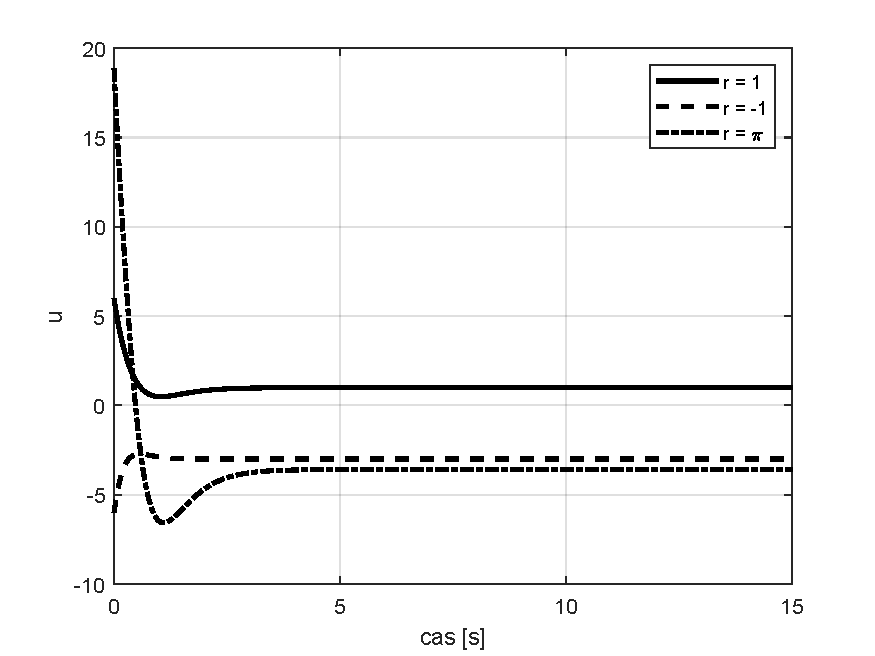
\includegraphics[width=1\linewidth]{u.pdf}
     \caption{Priebeh akčného zásahu $u$ s nelineárnym riadením}
	\label{fig:Vysledok2}
   \end{minipage}
\end{figure}

\subsubsection{Rovnovážne stavy systému}
V rovnovážnom stave sú derivácie rovné nule. Z rovníc \ref{eqn:RB} vyplýva, že bod $x_1 = x_2 = 0$ je rovnovážnym bodom.
\begin{equation}
\begin{aligned}
    \dot{x_1}|_{x_1 = x_2 = u = 0} &=  0 \\
\dot{x_2}|_{x_1 = x_2 = u = 0} &= 0 \\
\end{aligned}
\label{eqn:RB}
\end{equation}
\begin{figure}[H]
	\begin{center}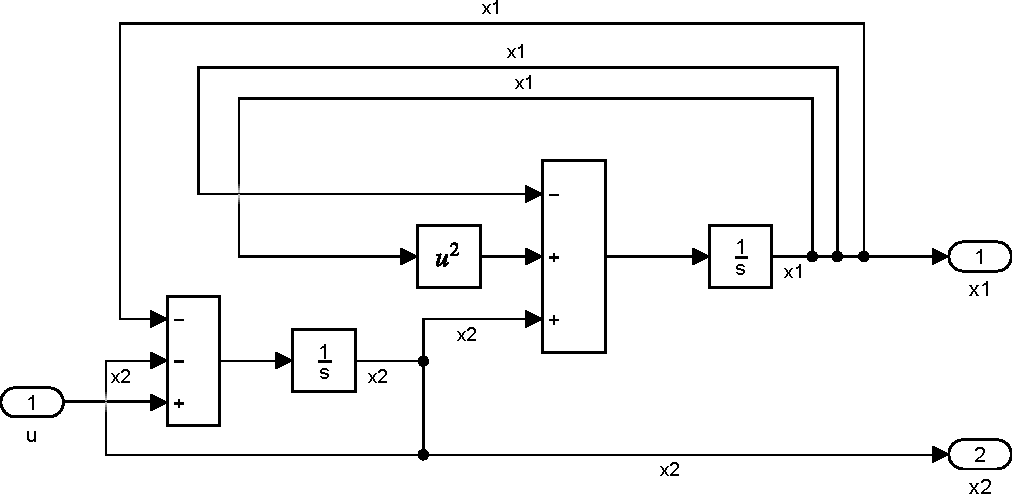
\includegraphics[scale=0.8]{Rovnica1.pdf}\end{center}
	\caption{Bloková schéma systému \ref{eqn:Rovnica1}}
	\label{fig:BlokovaSchemaPr1}
\end{figure}

\subsubsection{Návrh PID regulátora}
Teraz môžeme pre porovnanie navrhnúť PID regulátor. Aby sme mohli navrhnúť PID regulátor potrebujeme získať prenosovú funkciu systému, preto náš systém linearzijeme v pracovnom bode $x_1 = x_2 = 0$ (rovnica \ref{eqn:LS}).
\begin{equation}
\begin{split} 
\begin{bmatrix} \Delta \dot{x_1} \\ \Delta \dot{x_2} \end{bmatrix}  & = A\begin{bmatrix} \Delta {x_1} \\ \Delta {x_2} \\ \Delta u \end{bmatrix}
 \end{split}
 \label{eqn:LS}
\end{equation}	

Pričom matica $A$ má tvar:
\begin{equation}
\begin{aligned} 
 A  & = \begin{bmatrix} \frac{\partial \dot{x_1}}{\partial x_1}& \frac{\partial \dot{x_1}}{\partial x_2}& \frac{\partial \dot{x_1}}{\partial u} \\ \frac{\partial \dot{x_2}}{\partial x_1}&\frac{\partial \dot{x_2}}{\partial x_2} & \frac{\partial \dot{x_2}}{\partial u}\end{bmatrix}_{|_{x_1 = x_2 = u = 0}} \\
 & = \begin{bmatrix} 2x_1-1 & 1 & 0 \\ -1 & -1 & 1 \end{bmatrix}_{|_{x_1 = x_2 = u = 0}} \\
  & = \begin{bmatrix} -1 & 1 & 0 \\ -1 & -1 & 1 \end{bmatrix}_{|_{x_1 = x_2 = u = 0}} \
 \end{aligned}
 \label{eqn:AL}
\end{equation}	
Hľadané linearizované rovnice: 
\begin{equation}
\begin{aligned} 
\Delta \dot{x_1}  &= -\Delta x_1 + \Delta x_2 \\
\Delta \dot{x_2} & = -\Delta x_1 - \Delta x_2 + \Delta u \
 \end{aligned}
 \label{eqn:LR}
\end{equation}	

Keď sme získali linearizované rovnice nelineárneho systému, z ktorých vyjadríme prenosovú funkciu $\frac{\Delta x_1}{\Delta u}$.Použijeme Laplaceovú transformáciu, aby sme sa získali prenosovú funkciu (rovnica \ref{eqn:PF}).
\begin{equation}
\begin{aligned} 
s\Delta \dot{x_1}  &= -\Delta x_1 + \Delta x_2 => \Delta x_2 = \Delta x_1(s+1) \\
s\Delta \dot{x_2} & = -\Delta x_1 - \Delta x_2 + \Delta u \\\\
s\Delta x_1(s+1) & = -\Delta x_1 - \Delta x_1(s+1) + \Delta u\\
s\Delta x_1(s+1) + \Delta x_1 + \Delta x_1(s+1) & = \Delta u\\\\
\Delta u & = \Delta x_1(s^2+2s+2)\\\\
\frac{\Delta x_1}{\Delta u} & = \frac{1}{(s^2+2s+2)}\
 \end{aligned}
 \label{eqn:PF}
\end{equation}	

Na výpočet parametrov PID regulátora použijeme metódu Pole-Placement. Aby sme ju mohli použiť vyjadríme si charakteristický polynóm (N(s)) z prenosovej funkcie uzavretého regulačného obvodu ${G_{URO}}$ (rovnica \ref{eqn:GURO})
\begin{equation}
	\begin{aligned}
	G_{URO} &= \frac{(P+Ds+\frac{I}{s})(\frac{1}{s^2+2s+2})}{1+(P+Ds+\frac{I}{s})(\frac{1}{s^2+2s+2})}  \\
		N(s)	&= s^3+s^2(2+D)+s(2+P)+I
	\end{aligned}
	\label{eqn:GURO}
\end{equation}

Keď sme získali charakteristický polynóm N(s), využijeme  metódu Pole-Placement, ktorá spočíva v porovnaní charakteristického polynómu so želaným polynómom P(s). Umiestníme póly želaného polynómu P(s) do zápornej reálnej polroviny. My si zvolíme korene: $p_1 = -1$, $p_2 = -2$, $p_3 = -3$, čím zabezpečíme stabilitu lineárneho systému. Polynóm P(s) potom bude mať nasledujúci tvar (rovnica \ref{eqn:Ps}). 
\begin{equation}
	\begin{aligned}
	P(s) &= (s + 1)(s + 2)(s + 3) \\
		 &= s^3 + 6s^2 + 11s + 6 \\
	\end{aligned}
\label{eqn:Ps}
\end{equation}

Porovnaním želaného polynómu P(s) s charakteristickým polynómom N(s) \ref{eqn:PR_porovnanie}, dostaneme parametre regulátora \ref{eqn:PR}.
\begin{equation}
	\begin{aligned}
	P(s) &= N(s) \\
	s^3 + 6s^2 + 11s + 6 &= s^3+s^2(2+D)+s(2+P)+I\\
	\end{aligned}
 \label{eqn:PR_porovnanie}
\end{equation}	
 \begin{equation}
\begin{bmatrix}P \\I\\ D \end{bmatrix} = \begin{bmatrix} 9 \\6\\4 \end{bmatrix}
 \label{eqn:PR}
\end{equation}

Výsledky overíme simulačne pomocou schémy na obrázku \ref{fig:PrikladsRiadenimPID}.
\begin{figure}[H]
	\begin{center}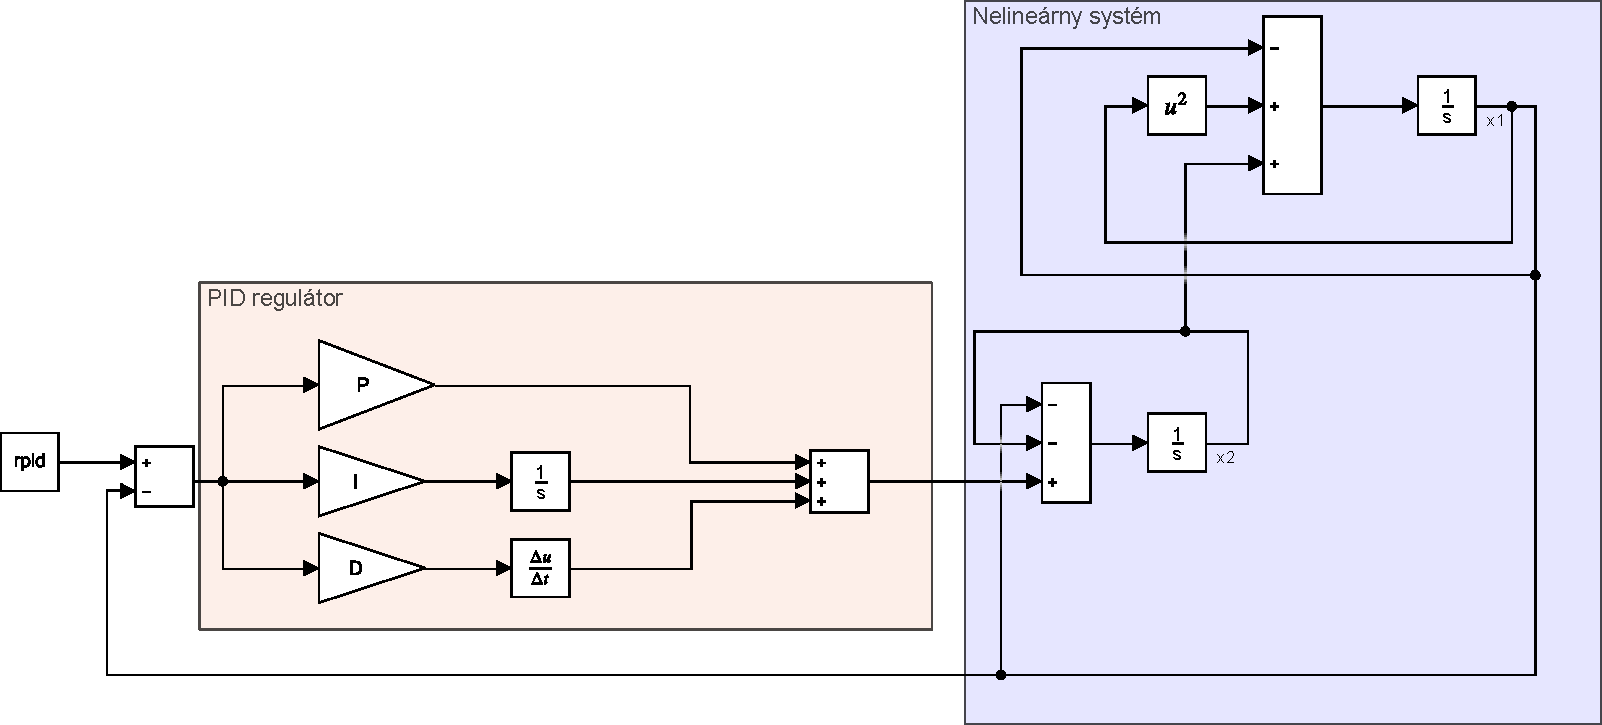
\includegraphics[scale=0.6]{pid.pdf}\end{center}
	\caption{Bloková schéma systému s PID regulátorom}
	\label{fig:PrikladsRiadenimPID}
\end{figure}

Z výsledkov simulácie, ktoré sú zobrazené na obrázkoch \ref{fig:Vysledok1}, \ref{fig:Vysledok2}, môžeme vidieť, že s pomocou PID regulátora sme dokázali dosiahnuť niektoré požadované hodnoty $r$, avšak pri vyšších požadovaných hodnotách bol už systém nestabilný.
\begin{figure}[!htb]
   \begin{minipage}{0.46\textwidth}
     \centering
     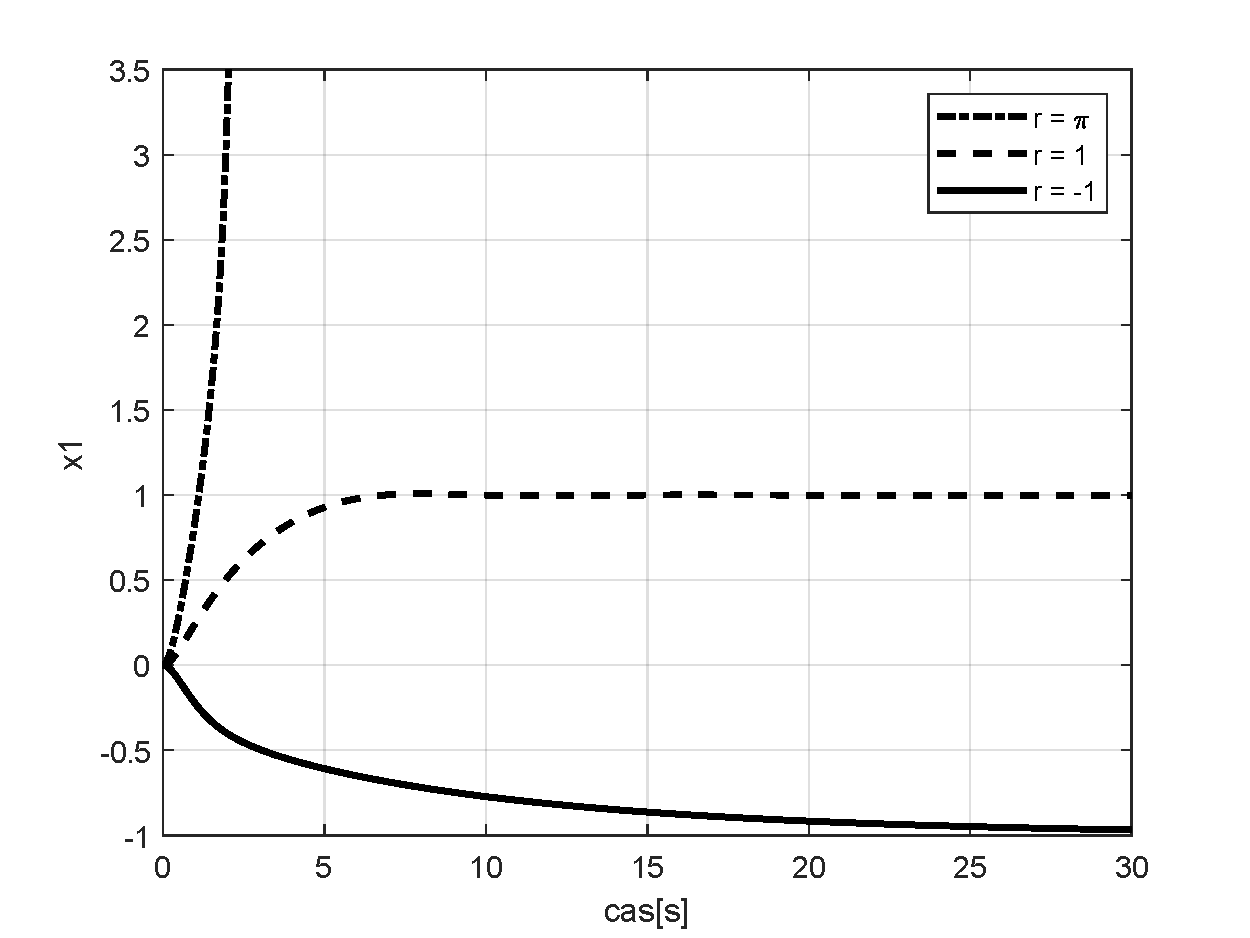
\includegraphics[width=1\linewidth]{xpid.pdf}
     \caption{Priebeh stavovej premennej $x_1$ s PID regulátorom}
	\label{fig:Vysledok1}
   \end{minipage}\hfill
   \begin{minipage}{0.46\textwidth}
     \centering
     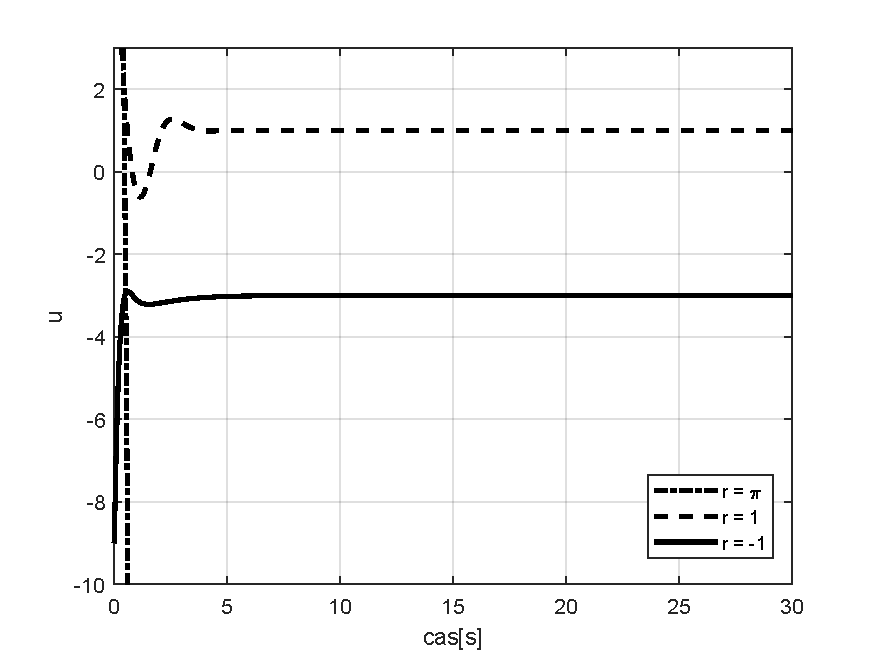
\includegraphics[width=1\linewidth]{upid.pdf}
     \caption{Priebeh akčného zásahu $u$ s PID regulátorom}
	\label{fig:Vysledok2}
   \end{minipage}
\end{figure}

\end{document}
